\documentclass[tikz,border=2pt]{standalone}
\usepackage{amsmath,amssymb}
\usepackage{pgfplots}
\pgfplotsset{compat=1.18}
\usetikzlibrary{arrows.meta}

\begin{document}
% Universality of the uniform: equally spaced probabilities u on the vertical axis, pushed
% through the quantile function Q = F^{-1}, land on the x-axis with density f: where F is
% steep the points crowd together. Conversely F(X) is uniform.
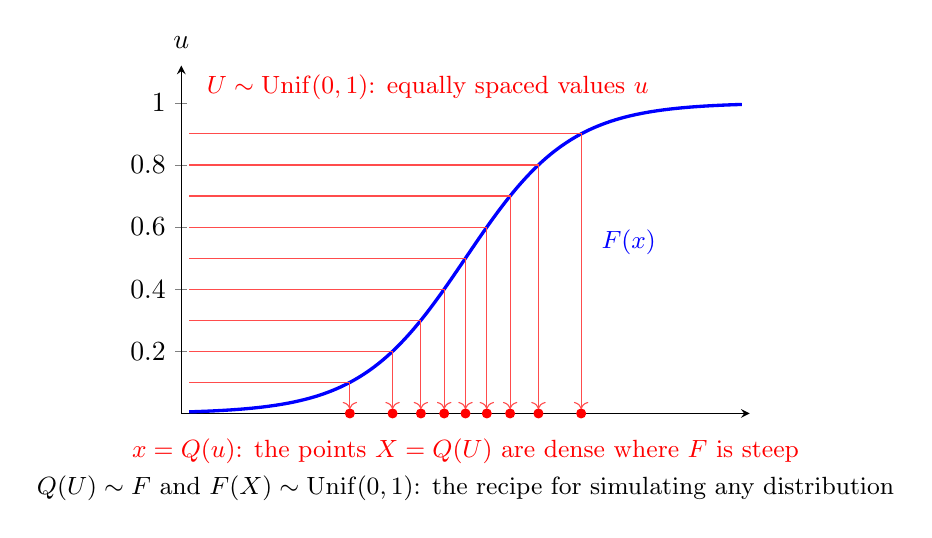
\begin{tikzpicture}
	\begin{axis}[
		axis lines=left, xmin=-3.6, xmax=3.6, ymin=0, ymax=1.12,
		xtick=\empty, ytick={0.2,0.4,0.6,0.8,1}, yticklabels={$0.2$,$0.4$,$0.6$,$0.8$,$1$},
		ylabel={$u$}, ylabel style={rotate=-90, anchor=south, at={(axis description cs:0,1.02)}},
		samples=140, smooth, width=8.8cm, height=6cm, clip=false
		]
		\addplot[blue, very thick, domain=-3.5:3.5] {1/(1+exp(-1.5*x))};
		\draw[red!70, thin, ->] (axis cs:-3.5,0.1) -- (axis cs:-1.465,0.1) -- (axis cs:-1.465,0.015);
		\draw[red!70, thin, ->] (axis cs:-3.5,0.2) -- (axis cs:-0.924,0.2) -- (axis cs:-0.924,0.015);
		\draw[red!70, thin, ->] (axis cs:-3.5,0.3) -- (axis cs:-0.565,0.3) -- (axis cs:-0.565,0.015);
		\draw[red!70, thin, ->] (axis cs:-3.5,0.4) -- (axis cs:-0.270,0.4) -- (axis cs:-0.270,0.015);
		\draw[red!70, thin, ->] (axis cs:-3.5,0.5) -- (axis cs:0,0.5) -- (axis cs:0,0.015);
		\draw[red!70, thin, ->] (axis cs:-3.5,0.6) -- (axis cs:0.270,0.6) -- (axis cs:0.270,0.015);
		\draw[red!70, thin, ->] (axis cs:-3.5,0.7) -- (axis cs:0.565,0.7) -- (axis cs:0.565,0.015);
		\draw[red!70, thin, ->] (axis cs:-3.5,0.8) -- (axis cs:0.924,0.8) -- (axis cs:0.924,0.015);
		\draw[red!70, thin, ->] (axis cs:-3.5,0.9) -- (axis cs:1.465,0.9) -- (axis cs:1.465,0.015);
		\addplot[only marks, red, mark=*, mark size=1.6pt] coordinates {(-1.465,0) (-0.924,0) (-0.565,0) (-0.270,0) (0,0) (0.270,0) (0.565,0) (0.924,0) (1.465,0)};
		\node[red, anchor=west, font=\small] at (axis cs:-3.4,1.05) {$U\sim \operatorname{Unif}(0,1)$: equally spaced values $u$};
		\node[red, anchor=north, font=\small] at (axis cs:0,-0.05) {$x=Q(u)$: the points $X=Q(U)$ are dense where $F$ is steep};
		\node[blue, anchor=west, font=\small] at (axis cs:1.6,0.55) {$F(x)$};
		\node[anchor=north, font=\small] at (axis cs:0,-0.17) {$Q(U)\sim F$ and $F(X)\sim \operatorname{Unif}(0,1)$: the recipe for simulating any distribution};
	\end{axis}
\end{tikzpicture}
\end{document}
